\chapter{Discussion}



\section{Application}

\subsection{Home application}

\subsection{Monitor}

\subsection{Main application}



\subsection{Indoor}
The aim of this section is to shortly investigate the wave behaver of the speaker array inside with wall reflection. This project have covered the design of the beamforming array and the behaver in free field condition. The indoor application have been keep out of interest, because of the starting point of application, which have been focused on outdoor event. The last point in the introduction was questioning the indoor application of the beamforming array. At this point there is many possibility since every room is different. The room could be a big concert hall or just a small room for living. It have been chosen to simulate a concert hall because of the monitoring application and the living room for home application. For the living room, it have been chosen to use a standard listening room of size (\SI{4.15}{\meter} x \SI{7.8}{\meter}) which correspond to the \gls{aau} standard listening room. All simulation will be done in 2 dimension because of the computation time and memory requirement. It will not give the exact simulation of the room, but since the reflection coefficient of the room wall not is measured there is already many unknown parameters in this simulation. Therefore the simulation give an impression of the wave behaviour in the room and not valid result. The result from a simulation of a size like the listening room is shown in \autoref{fig:Indoor_simulation_60_100} and \autoref{fig:Indoor_simulation_200_300}



\begin{figure}[H]
\begin{subfigure}[c]{0.5\textwidth}
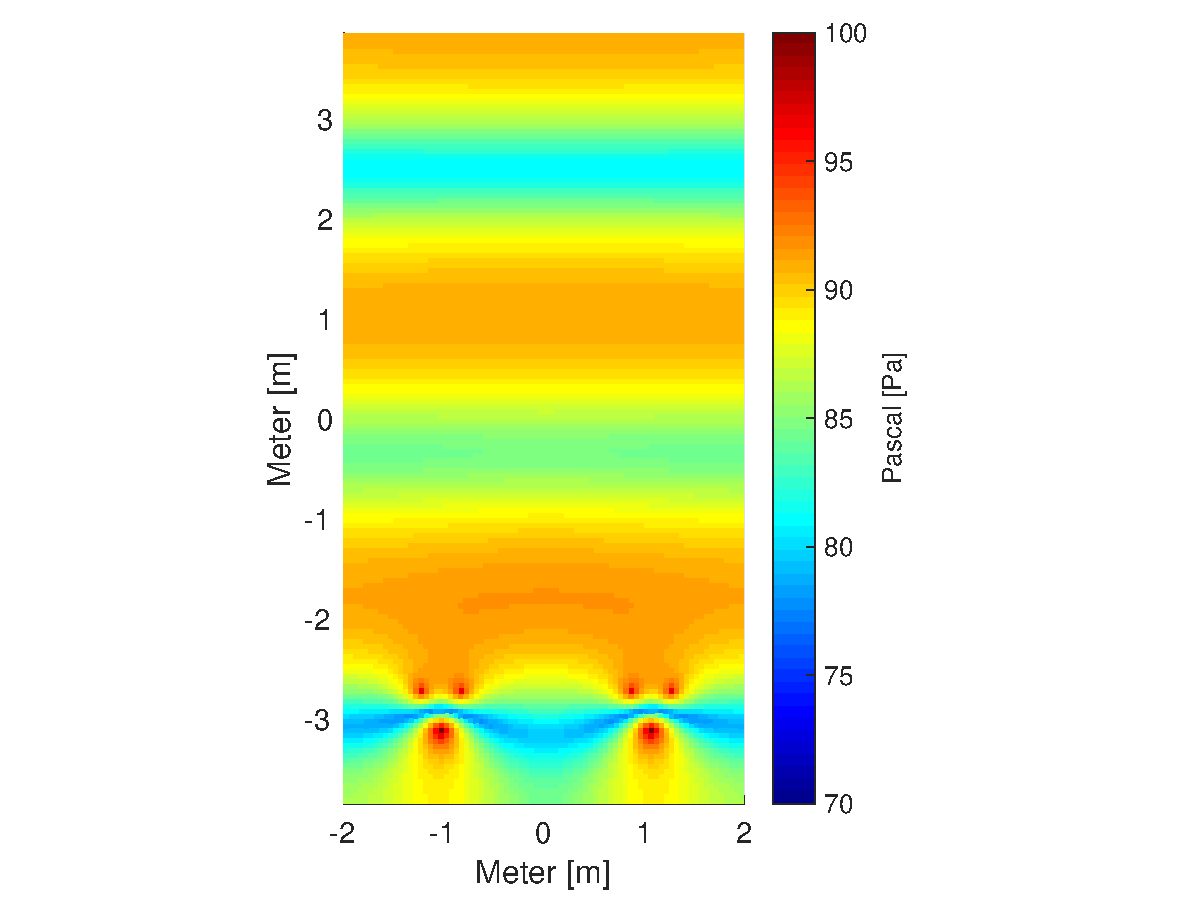
\includegraphics[width=0.95\textwidth]{60_hz_inside_beam.eps}
\subcaption{Indoor simulation of  \SI{60}{\hertz} with beamforming}
\label{fig:Indoor_simulation_60_on}
\end{subfigure}
\begin{subfigure}[c]{0.5\textwidth}
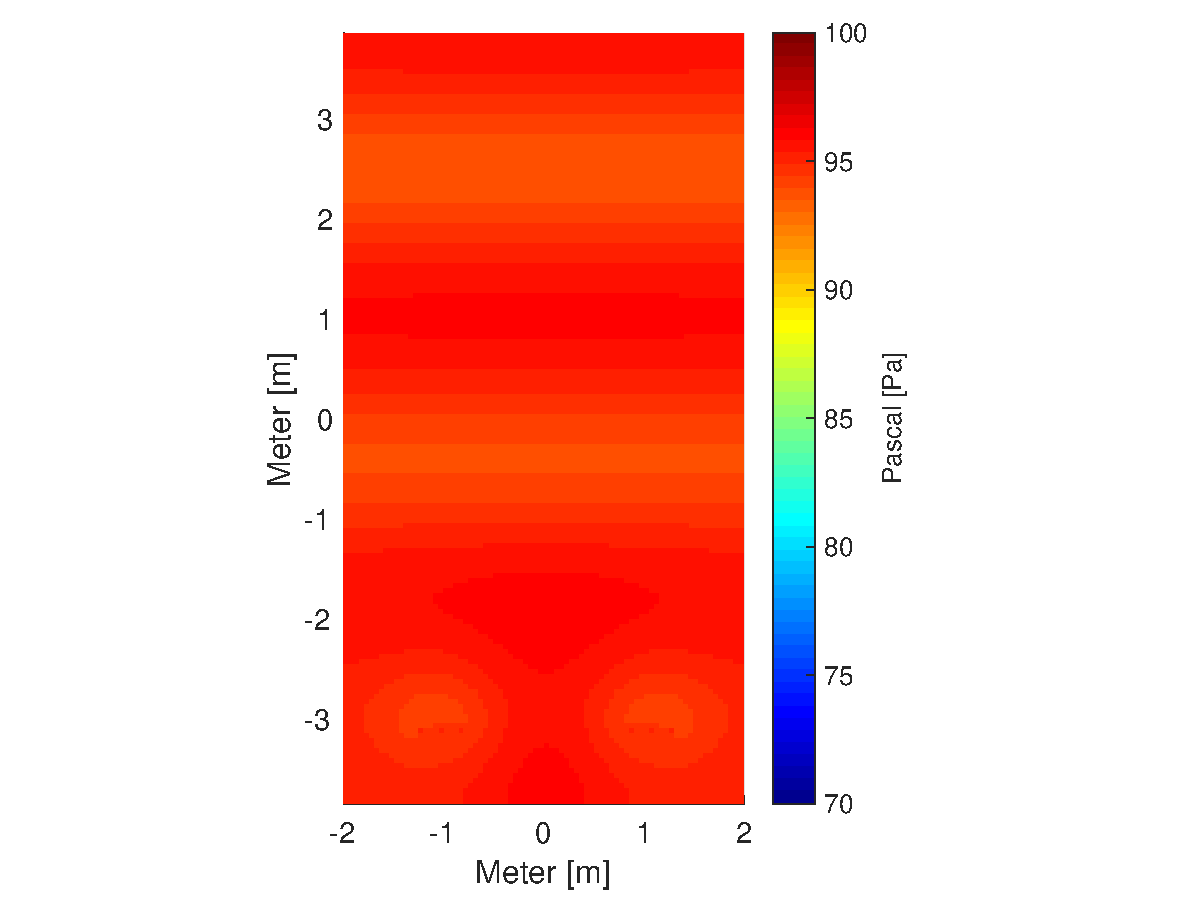
\includegraphics[width=0.95\textwidth]{60_hz_inside_without_beam.eps}
\subcaption{Indoor simulation of  \SI{60}{\hertz} without beamforming}
\label{fig:Indoor_simulation_60_off}
\end{subfigure}\\
\hspace{0.1\textheight}
\begin{subfigure}[c]{0.5\textwidth}
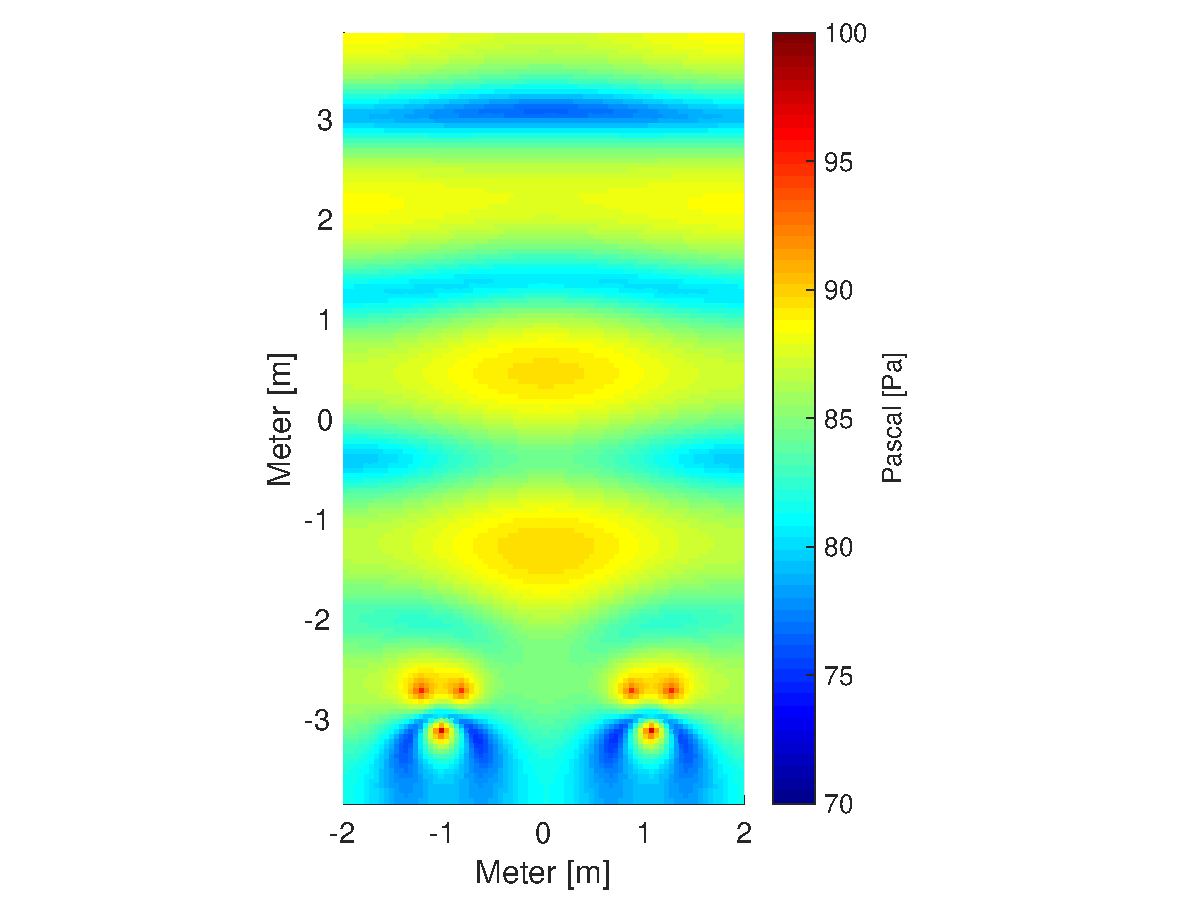
\includegraphics[width=0.95\textwidth]{100_hz_inside_beam.eps}
\subcaption{Indoor simulation of  \SI{100}{\hertz} with beamforming}
\label{fig:Indoor_simulation_100_on}
\end{subfigure}
\begin{subfigure}[c]{0.5\textwidth}
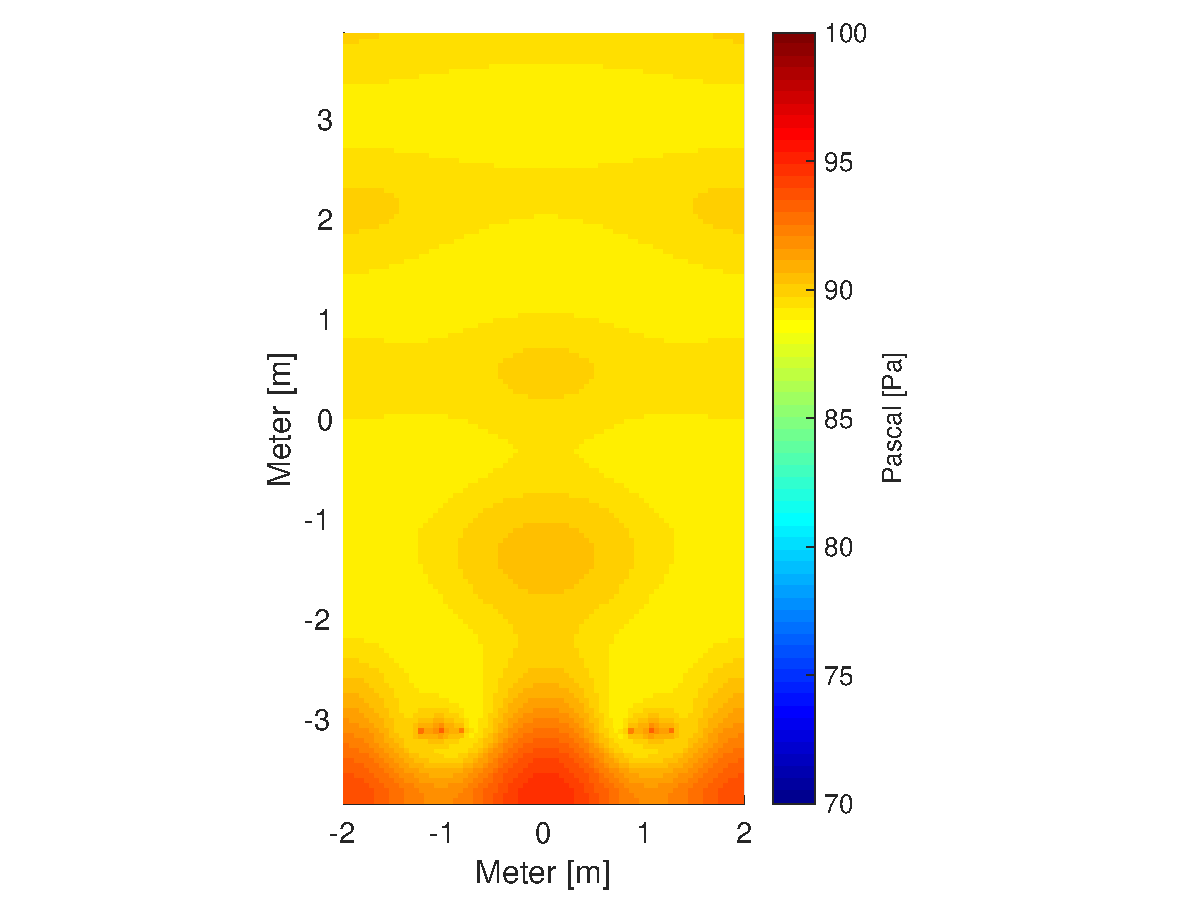
\includegraphics[width=0.95\textwidth]{100_hz_inside_without_beam.eps}
\subcaption{Indoor simulation of  \SI{100}{\hertz} with beamforming}
\label{fig:Indoor_simulation_100_off}
\end{subfigure}
\caption{The figure shows a 2 dimension \gls{fdtd} simulation in a standard listening room}
		\label{fig:Indoor_simulation_60_100}
\end{figure}


\begin{figure}[H]
\begin{subfigure}[c]{0.5\textwidth}
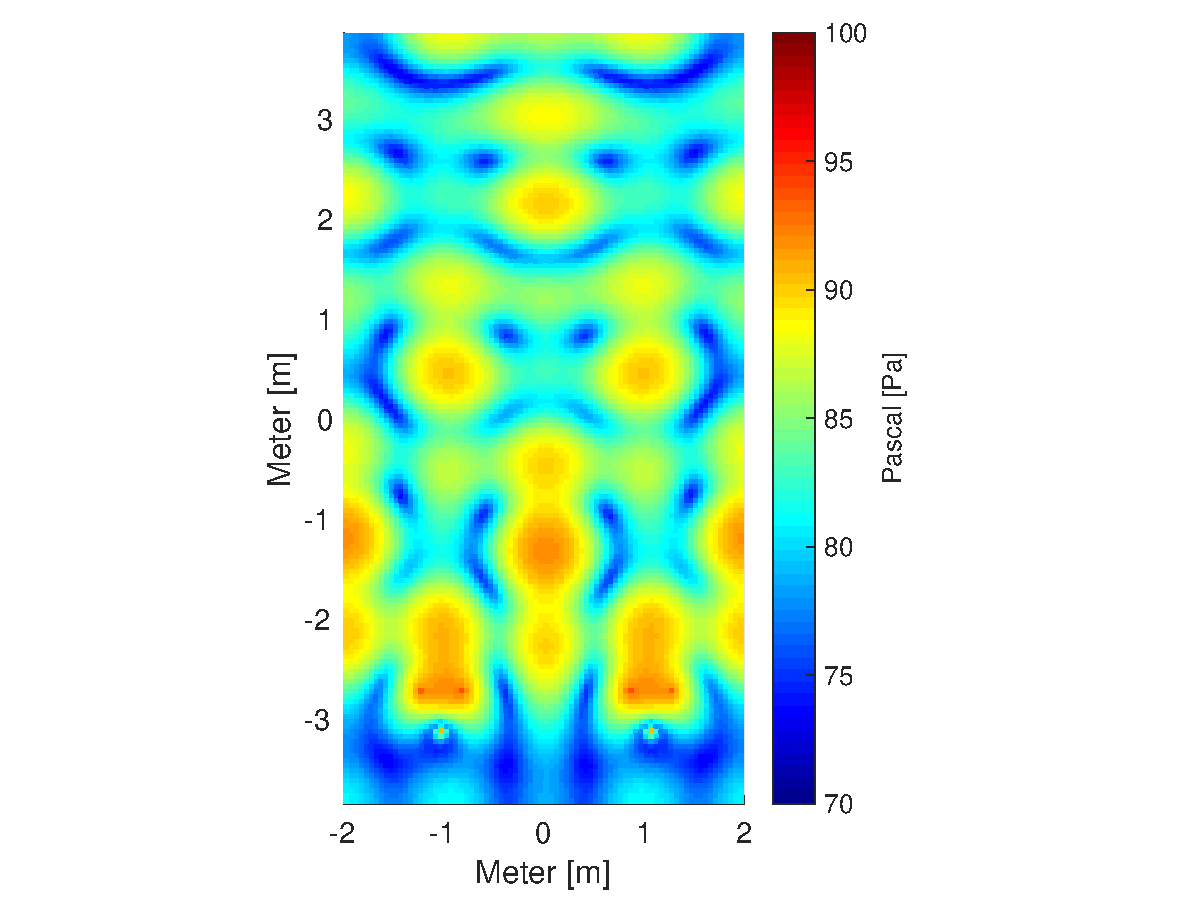
\includegraphics[width=0.95\textwidth]{200_hz_inside_beam.eps}
\subcaption{Indoor simulation of  \SI{200}{\hertz} with beamforming}
\label{fig:Indoor_simulation_200_on}
\end{subfigure}
\begin{subfigure}[c]{0.5\textwidth}
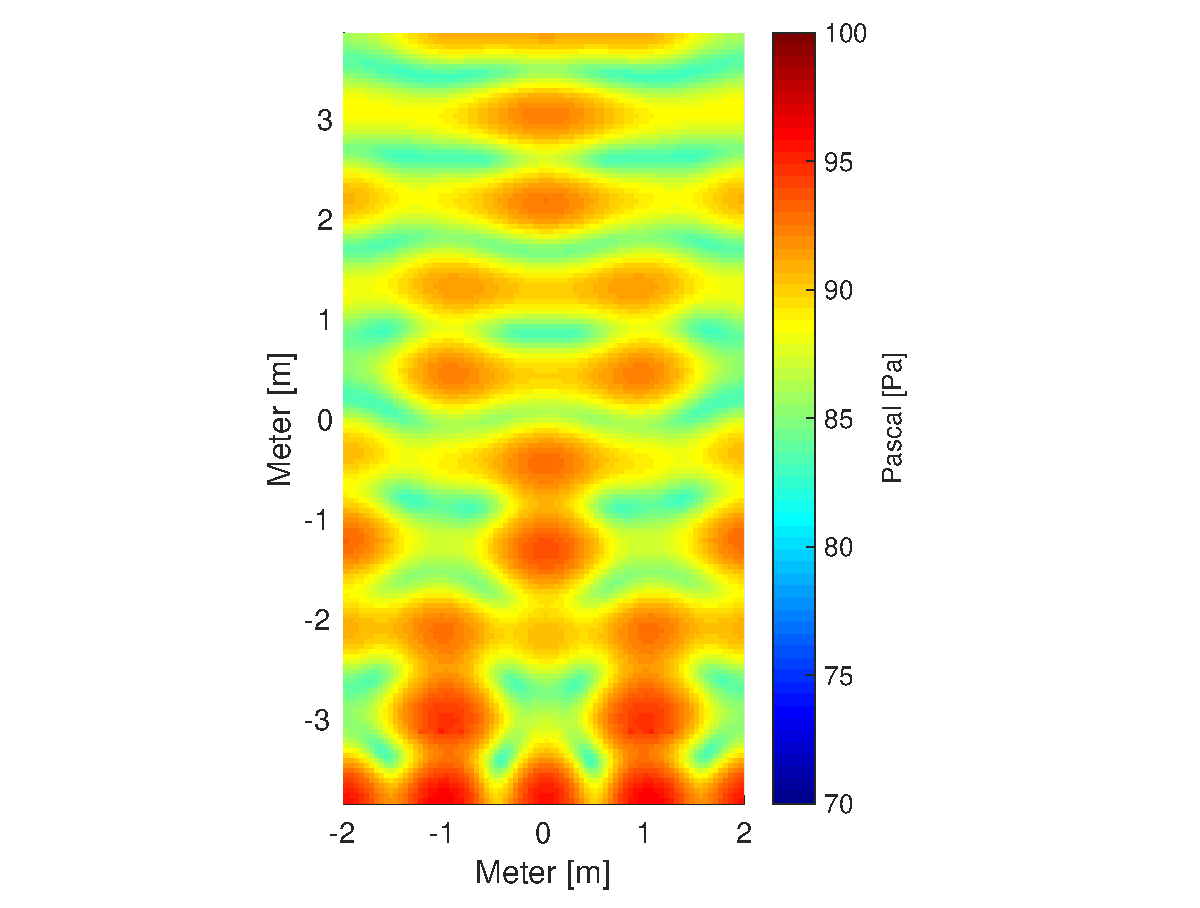
\includegraphics[width=0.95\textwidth]{200_hz_inside_without_beam.eps}
\subcaption{Indoor simulation of  \SI{200}{\hertz} without beamforming}
\label{fig:Indoor_simulation_200_off}
\end{subfigure}
\begin{subfigure}[c]{0.5\textwidth}
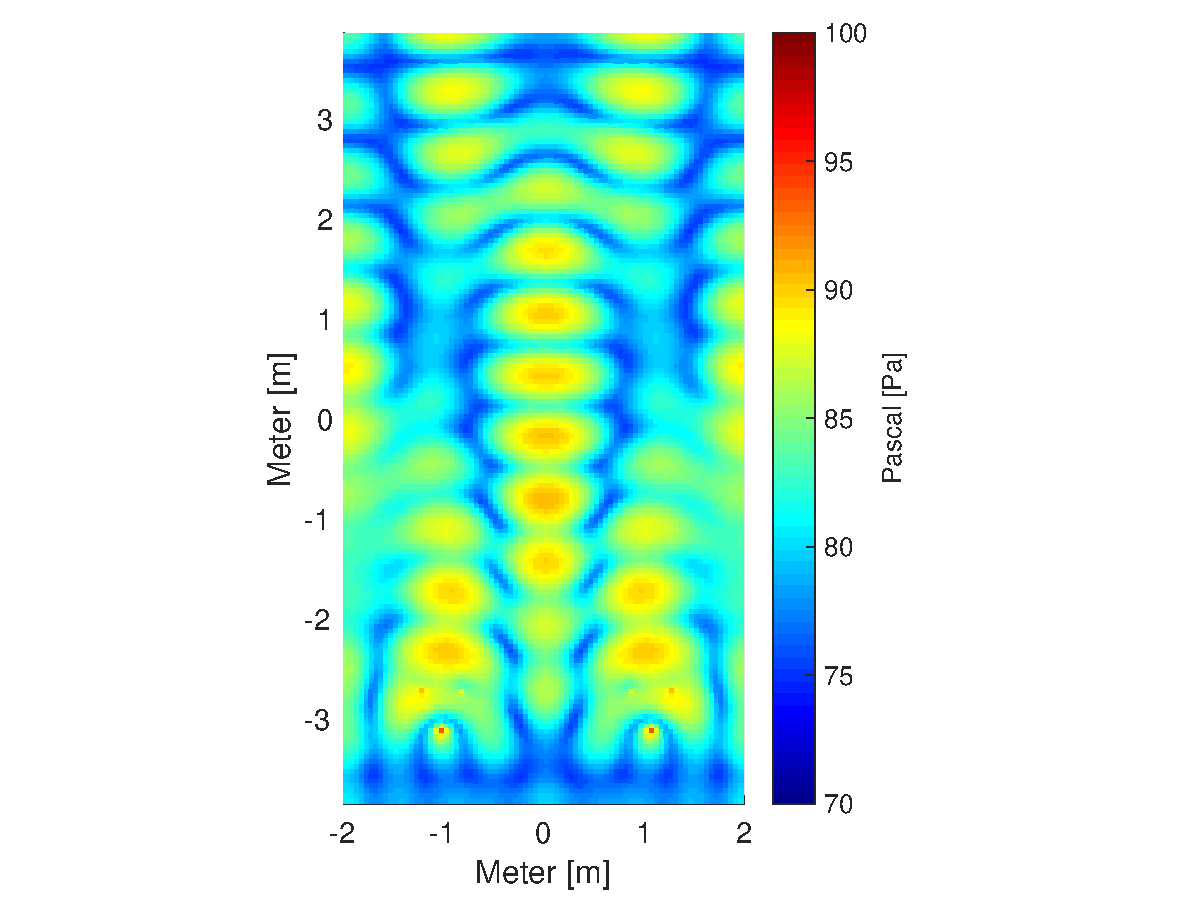
\includegraphics[width=0.95\textwidth]{300_hz_inside_beam.eps}
\subcaption{Indoor simulation of  \SI{300}{\hertz} with beamforming}
\label{fig:Indoor_simulation_300_on}
\end{subfigure}
\begin{subfigure}[c]{0.5\textwidth}
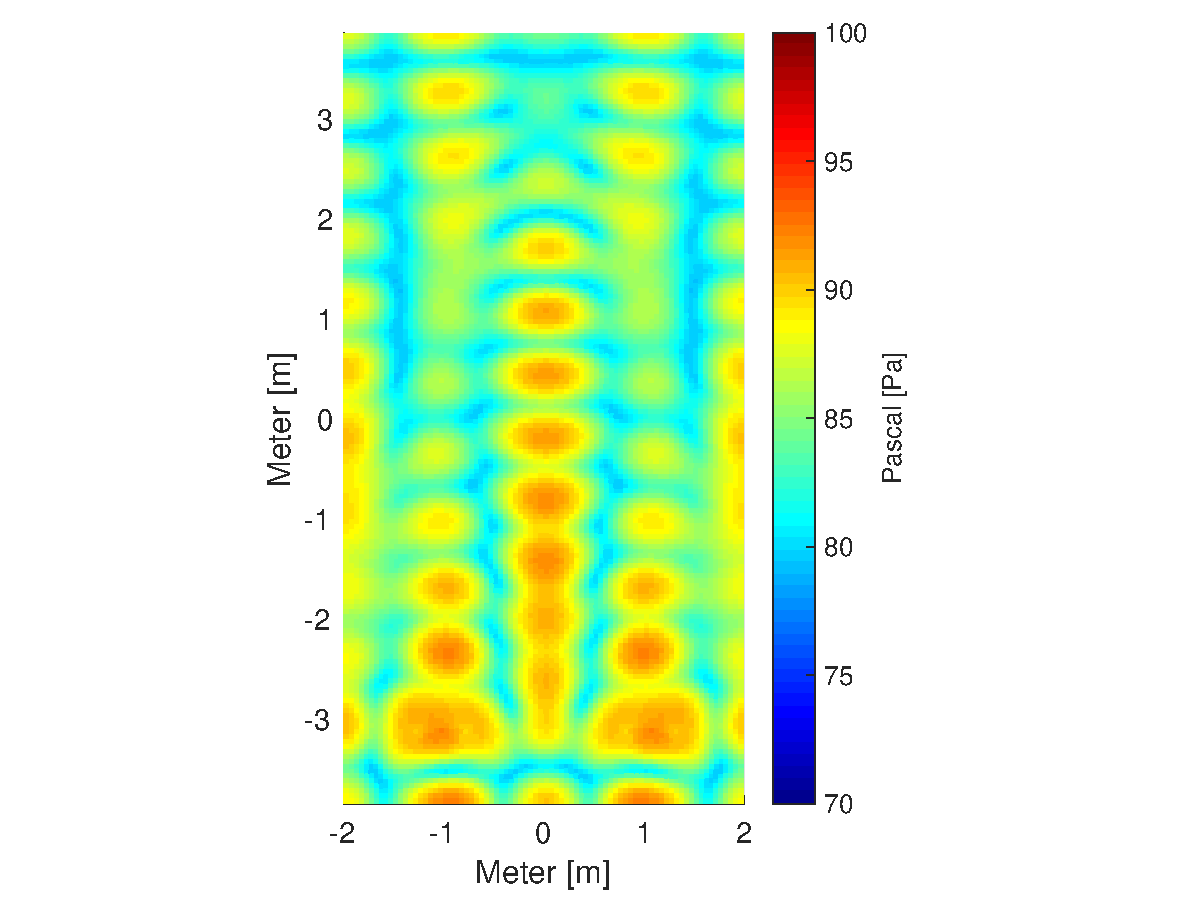
\includegraphics[width=0.95\textwidth]{300_hz_inside_without_beam.eps}
\subcaption{Indoor simulation of  \SI{300}{\hertz} without beamforming}
\label{fig:Indoor_simulation_300_off}
\end{subfigure}
\caption{The figure shows \gls{fdtd} simulation in between the used frequency range for polar plot in this project.}
		\label{fig:Indoor_simulation_200_300}
\end{figure}

In \autoref{fig:Indoor_simulation_60_100} and \autoref{fig:Indoor_simulation_200_300} it can be seen that the pressure in the room is not even ether with beamforming active or not. But one notable thing is that the pressure in the room at low frequency with omnidirectional array gets very high compare to higher frequency. So the room amplify the low frequency with reflection more that in the higher frequency area. The pressure seems to be more frequency pressure constant with beamforming active compare to beamforming disabled.\\


A second indoor application is the monitoring. In a monitoring application the room tens to be larger than a living room. The use of monitoring is often to both small and big concert where both dedicated concert hall and sports arenas are used. The following simulating example are done in a sports arena where the spectator area are on the long side of the playing field. An handball playing field do have a size of (\SI{20}{\meter}x\SI{40}{\meter}) and in this case the spectator is \SI{5}{\meter} on both long side. The following simulation \autoref{fig:Indoor_monitor_60_300} shows a simulation where the stage is placed on the top of the simulation with two monitor. Both monitors is playing upwards when looking at the simulation.


\begin{figure}[H]
\begin{subfigure}[c]{0.5\textwidth}
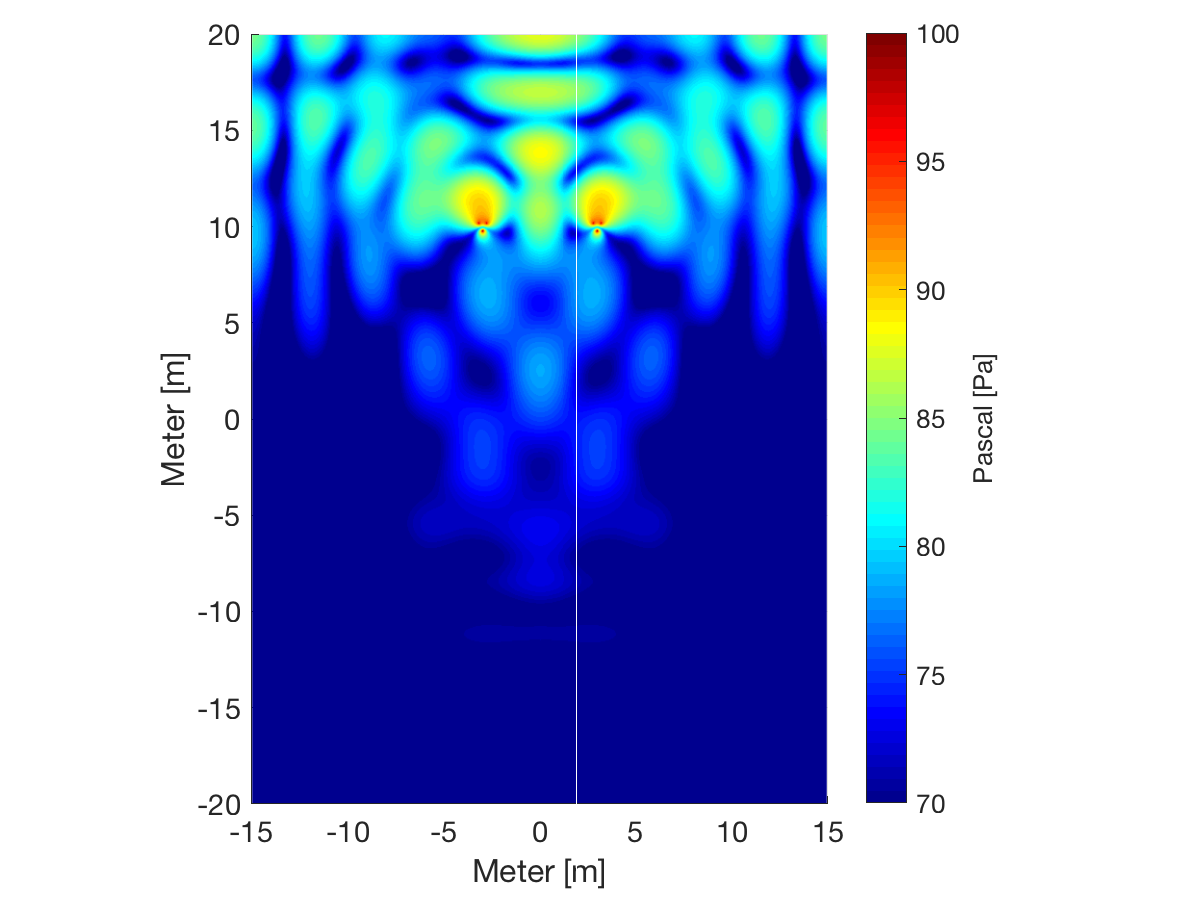
\includegraphics[width=0.95\textwidth]{60_hz_monitor_beam.eps}
\subcaption{Indoor simulation of  \SI{60}{\hertz} with beamforming}
\label{fig:Indoor_monitor_60_on}
\end{subfigure}
\begin{subfigure}[c]{0.5\textwidth}
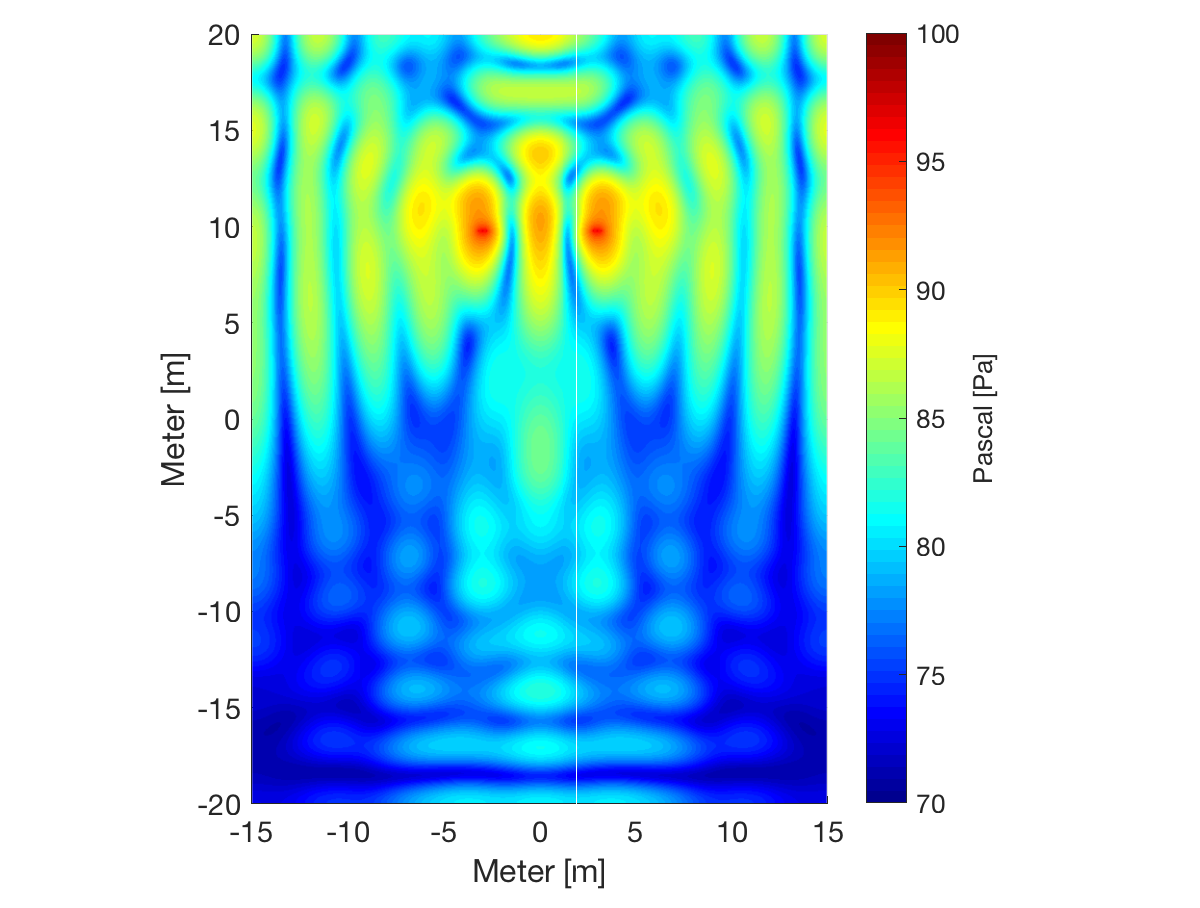
\includegraphics[width=0.95\textwidth]{60_hz_monitor_without_beam.eps}
\subcaption{Indoor simulation of  \SI{60}{\hertz} without beamforming}
\label{fig:Indoor_monitor_60_off}
\end{subfigure}\\
\hspace{0.1\textheight}
\begin{subfigure}[c]{0.5\textwidth}
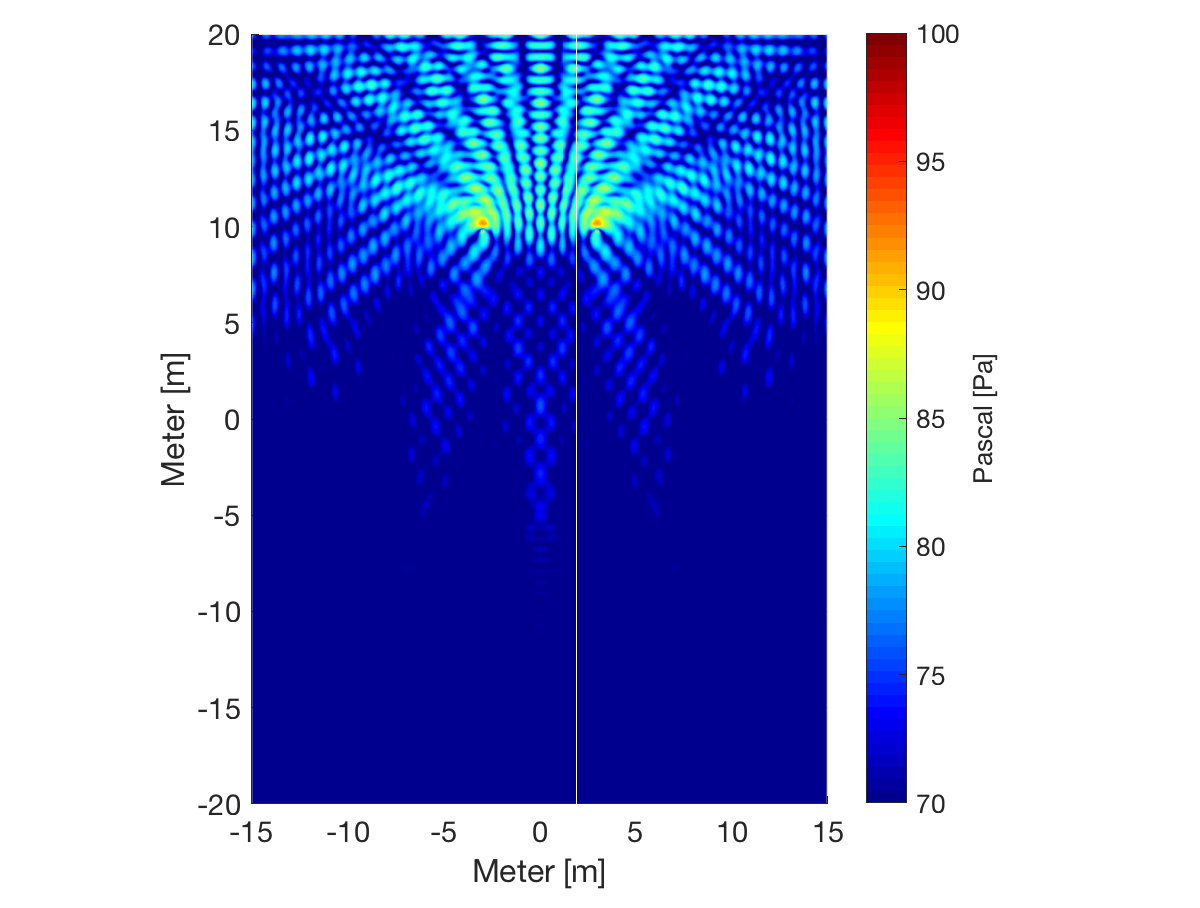
\includegraphics[width=0.95\textwidth]{300_hz_monitor_beam.eps}
\subcaption{Indoor simulation of  \SI{100}{\hertz} with beamforming}
\label{fig:Indoor_monitor_300_on}
\end{subfigure}
\begin{subfigure}[c]{0.5\textwidth}
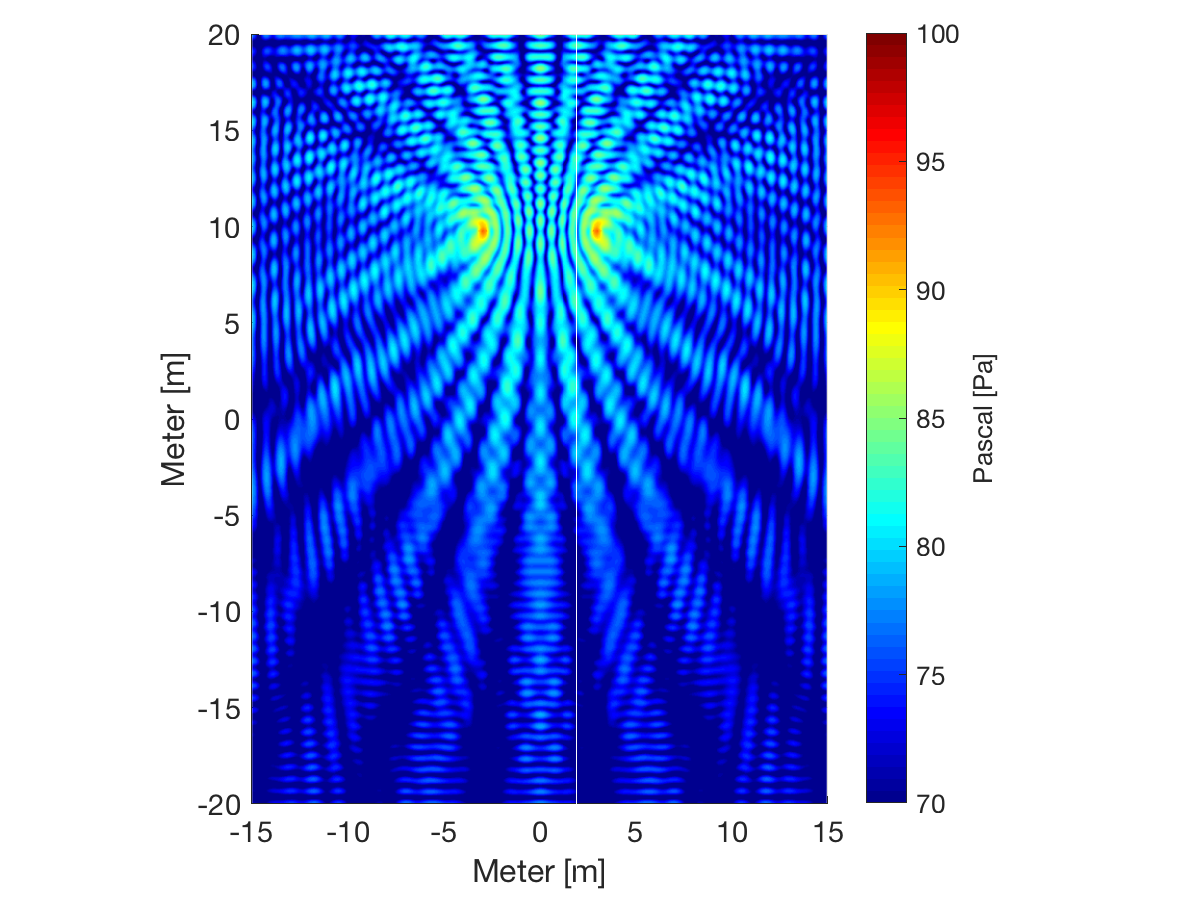
\includegraphics[width=0.95\textwidth]{300_hz_monitor_without_beam.eps}
\subcaption{Indoor simulation of  \SI{100}{\hertz} with beamforming}
\label{fig:Indoor_monitor_300_off}
\end{subfigure}
\caption{The figure shows a 2 dimension \gls{fdtd} simulation in a standard listening room}
		\label{fig:Indoor_monitor_60_300}
\end{figure}